\documentclass[11pt]{article}

\usepackage[margin=1in]{geometry}
\usepackage{amsmath, amssymb}
\usepackage{booktabs}
\usepackage{graphicx}
\usepackage{subcaption}
\usepackage{float}
\usepackage{array}
\usepackage{hyperref}
\usepackage{xcolor}
\usepackage{tikz}
\usetikzlibrary{arrows.meta, positioning, shapes.geometric, fit, backgrounds, calc}

\title{Oracle Belief Setup:\\
       Bounding the Value of Regime Information\\[0.4em]
       \large Belief-Aware RL Project --- Design Report v5}
\author{Belief-Aware RL Project}
\date{May 2026}

\begin{document}
\maketitle
\tableofcontents
\bigskip

% ---------------------------------------------------------------------------
\section{Motivation}
% ---------------------------------------------------------------------------

The sweep results in v1 and v4 establish a clear structural fact: which
trading strategy performs best depends on the hidden composition of
background agents, specifically the \emph{ratio of momentum followers to
value agents}.

\begin{itemize}
  \item At \texttt{num\_momentum\_agents}${}=0$, \texttt{num\_value\_agents}${}=102$
        (ratio $r=0$): the \textsc{Value}/MR heuristic earns a median P\&L of
        $+328$ cents while the \textsc{Momentum} heuristic loses $-1{,}967$
        cents (v4, Table~2).
  \item At \texttt{num\_momentum\_agents}${}=12$, \texttt{num\_value\_agents}${}=102$
        (ratio $r\approx 0.12$, the default AAPL calibration): \textsc{Momentum}
        earns $+1{,}690$ cents while \textsc{Value} loses $-2{,}485$ cents
        (v4, Table~2). The \textsc{Momentum} heuristic also achieves a mean
        P\&L of $+66{,}172$ cents and an 82\% win rate over 50 episodes in
        the standalone baseline (v1, Table~3).
  \item At ratio $r\approx 0.49$ ($n_\mathrm{mom}=50$): both heuristics suffer
        catastrophic losses, indicating the regime has collapsed into a
        feedback-trading spiral that is harmful to all simple strategies.
\end{itemize}

\noindent
This is the necessary and sufficient condition for a belief-aware agent to
have an advantage: \emph{different regimes reward different actions, and the
agent observes neither the regime nor the agent counts directly.}
The oracle setup formalizes this advantage as a testable upper bound.

% ---------------------------------------------------------------------------
\section{Existing Data Supporting the Oracle Design}
\label{sec:existing}
% ---------------------------------------------------------------------------

\subsection{v4 PPO baseline (comparison target)}

The belief-blind PPO agent trained on the default AAPL calibration
($n_\text{mom}=12$, $n_\text{val}=102$) across two seeds produces the
metrics in Table~\ref{tab:v4baseline}.
These numbers are the \emph{pass/fail threshold} for all oracle experiments.

\begin{table}[H]
\centering
\begin{tabular}{lrrrrr}
\toprule
\textbf{Quantity} & \textbf{Seed 0} & \textbf{Seed 1} & \textbf{Avg.} \\
\midrule
Mean final P\&L (cents) & $30{,}528$ & $35{,}179$ & $32{,}854$ \\
Std.\ final P\&L (cents) & $11{,}353$ & $15{,}135$ & --- \\
Sharpe ratio             & $2.689$    & $2.324$    & $2.507$   \\
Win rate                 & $1.00$     & $1.00$     & $1.00$    \\
Mean max drawdown        & $0.00298$  & $0.00341$  & $0.00320$ \\
\midrule
Timestep / episode length & \multicolumn{3}{c}{60\,s / 386 steps} \\
Eval episodes per seed    & \multicolumn{3}{c}{20} \\
\bottomrule
\end{tabular}
\caption{v4 belief-blind PPO baseline. Source:
         \texttt{results/ppo\_baseline/seed\_\{0,1\}/eval\_metrics.json}.
         A third seed aborted during training; two-seed averages are
         used throughout.}
\label{tab:v4baseline}
\end{table}

\subsection{Regime separation: targeted heuristic sweep}

The targeted sweep (\texttt{targeted\_sweep.json}; $n=10$ episodes per cell,
300\,s timestep / 78-step episodes) varies \texttt{num\_momentum\_agents}
while holding $n_\text{val}=102$ and all other parameters at default.
Table~\ref{tab:sweepregime} shows results for the two strategies directly
relevant to the oracle design.

\begin{table}[H]
\centering
\begin{tabular}{lrrrr}
\toprule
& \multicolumn{2}{c}{\textbf{VALUE strategy}} &
  \multicolumn{2}{c}{\textbf{MOMENTUM strategy}} \\
\cmidrule(lr){2-3}\cmidrule(lr){4-5}
$n_\text{mom}$ & Median P\&L & Win \% & Median P\&L & Win \% \\
\midrule
$0$  \textit{(Val regime)}  & $+328$        & 50 & $-1{,}967$       & 30 \\
$12$ \textit{(Mom regime)}  & $-2{,}484$    & 30 & $+1{,}690$       & 60 \\
$50$ \textit{(excluded)}    & $-344{,}390$  & 50 & $-1{,}561{,}646$ & 0  \\
\bottomrule
\end{tabular}
\caption{Heuristic strategy performance by momentum-agent count.
         All P\&L values in cents; 300\,s timestep, 10 episodes per cell.
         Timed-out episodes omitted for $n_\text{mom}=50$.
         Source: \texttt{targeted\_sweep.json}.}
\label{tab:sweepregime}
\end{table}

\paragraph{Key observations.}
\begin{enumerate}
  \item \textbf{Regime reversal is confirmed.} At $n_\text{mom}=0$, VALUE
        outperforms MOMENTUM ($+328$ vs $-1{,}967$); at $n_\text{mom}=12$,
        MOMENTUM outperforms VALUE ($+1{,}690$ vs $-2{,}484$). The sign of
        the advantage flips cleanly between the two oracle regimes.
  \item \textbf{The extreme regime is excluded by design.} At
        $n_\text{mom}=50$ both strategies suffer catastrophic losses; there
        is no useful action signal to condition on, so this setting is not
        used as an oracle target.
  \item \textbf{Value-agent sweep is less clean.} Varying $n_\text{val}$
        while holding $n_\text{mom}=12$ fixed shows a weaker crossover:
        at $n_\text{val}=300$ both strategies lose (VALUE $-2{,}740$,
        MOMENTUM $-3{,}318$), consistent with over-anchoring collapsing the
        regime rather than creating a clean mean-reversion regime. The
        momentum-agent sweep is therefore the cleaner axis for defining
        oracle regimes.
\end{enumerate}

\subsection{E0 oracle heuristic estimate (sweep protocol)}
\label{sec:e0estimate}

Applying the oracle rule---play VALUE in \textsc{Val} episodes and MOMENTUM
in \textsc{Mom} episodes---to the existing sweep data gives an \emph{in-sweep}
estimate of oracle heuristic performance:

\begin{table}[H]
\centering
\begin{tabular}{lrrrr}
\toprule
\textbf{Condition} & \textbf{$n$} & \textbf{Mean P\&L} & \textbf{Sharpe} & \textbf{Win \%} \\
\midrule
Oracle heuristic (Val: VALUE, Mom: MOMENTUM) & 20 & $+1{,}182$ & $0.15$ & $55$ \\
Fixed MOMENTUM in both regimes              & 20 & $+647$     & $0.08$ & $45$ \\
\midrule
v4 PPO baseline (60\,s timestep)            & 40 & $+32{,}854$ & $2.51$ & $100$ \\
\bottomrule
\end{tabular}
\caption{Oracle heuristic estimate vs.\ v4 PPO baseline.
         \textbf{Warning:} heuristic rows use the 300\,s / 78-step sweep
         protocol; the v4 baseline uses the 60\,s / 386-step training
         protocol. Rows are \emph{not} directly comparable --- see
         Section~\ref{sec:protocolgap}.}
\label{tab:e0estimate}
\end{table}

\subsubsection{Evaluation-protocol gap}
\label{sec:protocolgap}

The oracle heuristic mean P\&L of $+1{,}182$ cents (Table~\ref{tab:e0estimate})
\emph{cannot} be compared directly to the v4 PPO baseline mean of $+32{,}854$
cents.
The two figures use different simulation protocols:

\begin{table}[H]
\centering
\begin{tabular}{lrr}
\toprule
\textbf{Setting} & \textbf{Sweep (heuristic)} & \textbf{PPO baseline} \\
\midrule
Timestep duration  & 300\,s  & 60\,s \\
Steps per episode  & 78      & 386   \\
Episodes per cell  & 10      & 20 \\
Train seeds        & ---     & 2 \\
\bottomrule
\end{tabular}
\caption{Protocol differences between the targeted sweep and v4 PPO training.}
\label{tab:protocolgap}
\end{table}

Fewer steps per episode means fewer opportunities to earn (or lose) P\&L.
A rough linear scaling suggests the heuristic numbers should be multiplied by
$386/78 \approx 5$ before comparing---but the relationship is nonlinear
because large trending moves may be truncated at 78 steps.
The proper E0 test (Section~\ref{sec:testing}, step~1) must rerun the oracle
heuristic under the \emph{same 60\,s / 386-step protocol} used by v4.

\paragraph{What the sweep does confirm.}
Protocol-corrected absolute P\&L aside, the sweep establishes two
protocol-independent facts: (a) the sign of the performance advantage flips
between regimes for both strategies, and (b) the VALUE strategy under the
oracle regime ($+328$ cents) already beats fixed MOMENTUM under the same
regime ($-1{,}967$ cents) within the same protocol.
These facts do not depend on the timestep, and they are sufficient to
justify running E0 under the 60\,s protocol.

% ---------------------------------------------------------------------------
\section{Research Question}
% ---------------------------------------------------------------------------

\begin{center}
\fbox{\parbox{0.88\linewidth}{\centering
\textbf{If the agent is given the true market composition as an
auxiliary input, does it outperform the belief-blind PPO baseline?}\\[4pt]
\small
If yes: regime information is worth estimating. Proceed to a learned belief
module that infers the composition from public market history.\\
If no: the observable market signal is already sufficient, and a belief
module adds no value.
}}
\end{center}

\medskip
We test this in two complementary ways, which we call the \textbf{two
oracle variants}:

\begin{enumerate}
  \item \textbf{Belief in observation.} Append the true regime belief tuple
        $b^* = (p_\text{val},\, p_\text{mom})$ to the observation vector.
        The policy learns to use the ground-truth composition signal.
  \item \textbf{Belief in reward.} Shape the step reward with a
        regime-alignment bonus that rewards the agent for taking actions
        consistent with the oracle regime. The base reward function is
        unchanged; only the training signal is augmented.
\end{enumerate}

\noindent
If \emph{either} variant beats the v4 PPO baseline on both mean P\&L and
Sharpe ratio, the case for building a learned belief estimator is
established.

% ---------------------------------------------------------------------------
\section{Oracle Regime Configurations}
\label{sec:regimes}
% ---------------------------------------------------------------------------

\subsection{Regime selection rationale}

We restrict the oracle to \textbf{two regimes} derived directly from the
existing sweep data, avoiding any new simulation runs unless the two-regime
result is ambiguous.

\begin{table}[H]
\centering
\begin{tabular}{llrrrl}
\toprule
\textbf{Regime} & \textbf{Label} &
  $n_\text{mom}$ & $n_\text{val}$ & $r = n_\text{mom}/n_\text{val}$ &
  \textbf{Favored heuristic} \\
\midrule
Value-dominated  & \textsc{Val} & $0$  & $102$ & $0.000$ & MR / \textsc{Value} \\
Momentum-default & \textsc{Mom} & $12$ & $102$ & $0.118$ & \textsc{Momentum} \\
\bottomrule
\end{tabular}
\caption{Two oracle regime configurations. All other background parameters
         remain at the \texttt{rmsc04} AAPL calibration defaults.}
\label{tab:regimes}
\end{table}

\noindent
The extreme-momentum setting ($n_\text{mom}=50$, $r\approx 0.49$) is
deliberately excluded: both heuristics lose heavily (median Momentum P\&L
$=-1{,}561{,}646$ cents, v4 Table~2), meaning the regime provides no useful
action signal. An oracle over an incoherent regime is not a meaningful upper
bound.

\subsection{Oracle belief tuple}

In each episode the environment is instantiated under one of the two regimes
with equal probability:
$P(\text{Val}) = P(\text{Mom}) = 0.5$.
The oracle belief tuple $b^*$ is a probability vector over these two
classes:
\[
  b^* =
  \begin{cases}
    (1,\, 0) & \text{if episode is drawn from regime \textsc{Val},} \\
    (0,\, 1) & \text{if episode is drawn from regime \textsc{Mom}.}
  \end{cases}
\]
Under a hard oracle this is one-hot; under a soft oracle (used in the
reward-shaping variant) it could be a temperature-smoothed distribution.
For all v5 experiments we use the hard one-hot encoding. A soft version
is deferred to the inferred-belief stage, where the estimator will produce
calibrated probabilities rather than deterministic labels.

The tuple has dimension $2$ and is appended to the existing $7$-dimensional
observation vector produced by \texttt{markets-daily\_investor-v0},
producing an augmented observation of dimension $9$.

% ---------------------------------------------------------------------------
\section{Two Oracle Variants}
\label{sec:variants}
% ---------------------------------------------------------------------------

\subsection{Variant 1: belief in observation}

\paragraph{Setup.}
The observation fed to the PPO policy at every step is:
\[
  \tilde{o}_t = [o_t \;\|\; b^*],
  \qquad o_t \in \mathbb{R}^7,\; b^* \in \{0,1\}^2,\;
  \tilde{o}_t \in \mathbb{R}^9.
\]
The reward function is unchanged from the v4 PPO baseline (dense
mark-to-market increment, scaled by the environment).
The network architecture is the same as v4 (MLP policy).

\paragraph{What this tests.}
Whether the policy network can learn to condition its buy/hold/sell
decisions on the regime label. An agent that correctly uses $b^*$
should approach the performance of an oracle heuristic that always plays
\textsc{Momentum} in \textsc{Mom} episodes and MR in \textsc{Val}
episodes.

\paragraph{Expected outcome.}
Mean P\&L and Sharpe should be strictly higher than the v4 baseline
trained on the default AAPL calibration, because:
(a) the \textsc{Val} episodes now contribute positive MR P\&L instead of
the negative returns seen by a fixed momentum policy, and
(b) the joint training distribution is enriched with the value-dominated
regime, giving the policy experience at both ends of the ratio spectrum.

\subsection{Variant 2: belief in reward}

\paragraph{Setup.}
The observation is unchanged from the v4 baseline ($o_t \in \mathbb{R}^7$;
the agent does \emph{not} see $b^*$).
The training reward is augmented with a regime-alignment term:
\[
  \tilde{r}_t = r_t + \alpha \cdot \text{align}(a_t,\, b^*),
\]
where $\text{align}(a, b^*)$ is:

\begin{table}[H]
\centering
\begin{tabular}{lrr}
\toprule
Action $a_t$ &
  $\text{align}(a_t, \textsc{Val})$ &
  $\text{align}(a_t, \textsc{Mom})$ \\
\midrule
Buy  & $-1$ & $+1$ \\
Hold & $\phantom{-}0$ & $\phantom{+}0$ \\
Sell & $+1$ & $-1$ \\
\bottomrule
\end{tabular}
\caption{Regime-alignment bonus. The alignment encoding assumes:
         in \textsc{Val} episodes the agent should fade moves (sell on
         recent buys, buy on recent sells); in \textsc{Mom} episodes it
         should follow pressure (buy on upward imbalance).
         Note: the table gives a simplified per-action version; a
         more accurate alignment could condition on the observation as
         well.}
\label{tab:alignment}
\end{table}

\paragraph{Calibrating $\alpha$.}
The v4 baseline reports mean episode rewards of $7.8$--$9.0$ over $386$
steps, giving a typical \emph{per-step} reward magnitude of
$r_t \approx 0.018$--$0.023$.
With $\text{align} \in \{-1, 0, +1\}$, the shaping bonus is $\alpha \cdot
\text{align} \in [-\alpha, +\alpha]$.
To avoid the bonus dominating the P\&L signal:
\[
  \alpha \ll |r_t| \implies \alpha \ll 0.02
  \implies \alpha \lesssim 0.002.
\]
We therefore set $\alpha = 0.001$ as the default shaping coefficient.
A search over $\alpha \in \{10^{-4}, 10^{-3}, 10^{-2}\}$ should be run
once the training infrastructure is in place; $\alpha = 10^{-2}$ is the
practical upper bound beyond which the shaping term exceeds $r_t$ in
magnitude and begins to corrupt the P\&L credit signal.

\paragraph{What this tests.}
Whether the correct regime signal can be injected \emph{through credit
assignment} without the agent ever seeing the label at inference time.
If the shaped policy converges to a better policy, it suggests the MDP
reward signal alone is insufficient to distinguish regimes, and an
auxiliary signal is needed for training even if not for deployment.

\paragraph{Evaluation.}
At evaluation time the alignment bonus is removed; the agent is scored
solely on episode P\&L and Sharpe under the standard reward. This makes
the comparison to the v4 baseline fair.

% ---------------------------------------------------------------------------
\section{Experimental Protocol}
\label{sec:protocol}
% ---------------------------------------------------------------------------

\subsection{Training}

All oracle variants train for the same budget as v4: $200{,}000$ environment
timesteps, $16$ parallel runners, train batch size $2{,}000$, five PPO
epochs per batch, minibatch size $128$, learning rate $10^{-4}$, entropy
coefficient $0.01$.

Each variant is trained over \textbf{three seeds} (seeds $0$, $1$, $2$);
the failed third seed from v4 should be replicated here to achieve
three-seed parity.

During training, each episode is drawn from either the \textsc{Val} or
\textsc{Mom} regime with equal probability, independently for each of
the 16 parallel runners per batch.

\subsection{Evaluation}

Held-out evaluation uses \textbf{twenty episodes per regime per seed}
(40 episodes total per seed: 20 \textsc{Val} + 20 \textsc{Mom}), drawn
from evaluation seeds $100$--$119$ within each regime.
This separates the regime-specific performance from the aggregate.

\begin{table}[H]
\centering
\begin{tabular}{lll}
\toprule
\textbf{Condition} & \textbf{Obs dim} & \textbf{Reward} \\
\midrule
v4 PPO baseline (belief-blind) & $7$ & MtM increment \\
Oracle variant 1 (belief in obs) & $9$ & MtM increment \\
Oracle variant 2 (belief in reward) & $7$ & MtM increment $+$ $\alpha \cdot \text{align}$ (train only) \\
\bottomrule
\end{tabular}
\caption{Comparison conditions. All other hyperparameters are identical.}
\label{tab:conditions}
\end{table}

\subsection{Pass/fail gate}

The oracle experiment is declared successful---justifying the belief
estimator stage---if \emph{at least one variant} satisfies:
\begin{enumerate}
  \item Mean P\&L (aggregate across both regimes) $>$ v4 mean P\&L.
  \item Sharpe ratio $>$ v4 Sharpe ratio.
  \item Win rate $\ge$ v4 win rate.
\end{enumerate}
All three conditions must hold simultaneously. A variant that improves
P\&L but degrades Sharpe may indicate reward hacking rather than better
regime use.

% ---------------------------------------------------------------------------
\section{Testing Strategy}
\label{sec:testing}
% ---------------------------------------------------------------------------

\begin{figure}[H]
\centering
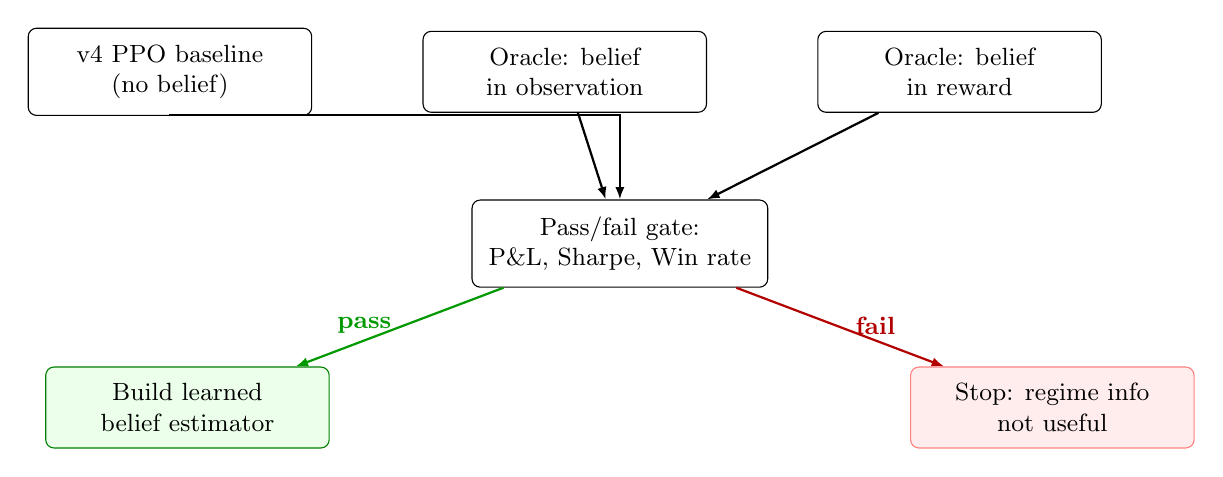
\begin{tikzpicture}[
  box/.style={draw, rounded corners=3pt, align=center, font=\small,
              minimum width=3.6cm, minimum height=0.8cm, inner sep=6pt},
  arr/.style={-{Latex[length=4.5pt]}, thick},
  grp/.style={draw=gray!40, rounded corners=6pt, inner sep=10pt, fill=gray!5},
  fail/.style={draw=red!50, fill=red!7},
  pass/.style={draw=green!50!black, fill=green!8},
]
  \node[box]                     (base) {v4 PPO baseline\\(no belief)};
  \node[box, right=1.4cm of base](obs)  {Oracle: belief\\in observation};
  \node[box, right=1.4cm of obs] (rew)  {Oracle: belief\\in reward};

  \node[box, below=1.1cm of obs, xshift=0.7cm] (gate)
        {Pass/fail gate:\\P\&L, Sharpe, Win rate};

  \draw[arr] (obs) -- (gate);
  \draw[arr] (rew) -- (gate);
  \draw[arr] (base) |- ++(0,-0.55) -| (gate);

  \node[box, pass, below left=1.0cm and 1.8cm of gate] (belief)
        {Build learned\\belief estimator};
  \node[box, fail, below right=1.0cm and 1.8cm of gate] (stop)
        {Stop: regime info\\not useful};

  \node[font=\small, green!60!black] at ($(gate)!0.5!(belief)+(-0.5,0)$) {\textbf{pass}};
  \node[font=\small, red!70!black]   at ($(gate)!0.5!(stop)+(0.5,0)$)   {\textbf{fail}};

  \draw[arr, green!60!black] (gate) -- (belief);
  \draw[arr, red!70!black]   (gate) -- (stop);
\end{tikzpicture}
\caption{Decision tree for the oracle experiment. Passing at least one
         variant unlocks the belief-estimator stage.}
\label{fig:decision}
\end{figure}

\subsection{Do we need to test it?}

Yes, for one specific reason: the oracle is the \emph{necessary} upper
bound check. Without it, the project cannot distinguish between two failure
modes:
\begin{enumerate}
  \item The learned belief module is insufficiently accurate.
  \item Regime information does not improve the policy at all (the
        observation signal already contains enough information for a
        fixed policy to perform well).
\end{enumerate}
If the oracle fails the gate, failure mode~(2) is the explanation and
there is no point training a belief module. If the oracle passes, failure
mode~(1) is the relevant direction and the gap between the oracle agent
and the learned-belief agent is the target to close.

\subsection{Step-by-step test plan}

\begin{enumerate}
  \item \textbf{Heuristic sanity check (no training, $\sim$15 min).}
        Implement an oracle heuristic: play \textsc{Momentum} if $b^*
        = (0,1)$ and play MR if $b^* = (1,0)$.
        Run 20 episodes per regime (40 total) under the \emph{60\,s /
        386-step} protocol.
        The sweep already confirms regime reversal in sign
        (Section~\ref{sec:e0estimate}); this step
        establishes absolute P\&L on the same footing as v4.
        \textbf{Status: pending} (sweep proxy exists; must rerun under
        60\,s protocol for direct v4 comparison).

  \item \textbf{Train oracle variant 1 (belief in obs, ~1.5 h per seed).}
        Augment the gym wrapper to append $b^*$ to observations.
        Train with three seeds, evaluate as described in
        Section~\ref{sec:protocol}. Compare against v4 per-seed and
        aggregate.

  \item \textbf{Train oracle variant 2 (belief in reward, ~1.5 h per seed).}
        Implement a shaped reward wrapper. Train with three seeds.
        Evaluate with the shaping \emph{removed} (standard reward only).

  \item \textbf{Apply pass/fail gate.} If either variant passes, proceed to
        the inferred-belief stage (Section~\ref{sec:next}).

  \item \textbf{Regime-stratified analysis.} Report metrics separately for
        \textsc{Val} episodes and \textsc{Mom} episodes. A well-functioning
        oracle agent should improve in both regimes; a confused agent may
        improve in one while degrading in the other.
\end{enumerate}

% ---------------------------------------------------------------------------
\section{Oracle Experiment Results}
\label{sec:results}
% ---------------------------------------------------------------------------

Table~\ref{tab:results_summary} is the central results table for v5.
Rows E0--E2 are filled in as experiments complete; E3 is the full
belief-aware agent that follows once the gate passes.

\begin{table}[H]
\centering
\begin{tabular}{llrrrrll}
\toprule
\textbf{Exp.} &
\textbf{Agent} &
\textbf{Mean P\&L} &
\textbf{Std P\&L} &
\textbf{Sharpe} &
\textbf{Win \%} &
\textbf{Gate} &
\textbf{Status} \\
\midrule
--- & v4 PPO baseline (60\,s) & $32{,}854$ & --- & $2.51$ & $100$ & \emph{target} & complete \\
\midrule
E0 & Oracle heuristic (60\,s) & \emph{TBD} & \emph{TBD} & \emph{TBD} & \emph{TBD} & \emph{TBD} & pending \\
E1 & PPO + belief in obs      & \emph{TBD} & \emph{TBD} & \emph{TBD} & \emph{TBD} & \emph{TBD} & pending \\
E2 & PPO + belief in reward   & \emph{TBD} & \emph{TBD} & \emph{TBD} & \emph{TBD} & \emph{TBD} & pending \\
E3 & PPO + inferred $\hat{b}$ & \emph{TBD} & \emph{TBD} & \emph{TBD} & \emph{TBD} & \emph{TBD} & blocked on E1/E2 \\
\bottomrule
\end{tabular}
\caption{Oracle experiment results summary.  Mean P\&L and Std in cents;
         Sharpe and Win\,\% are episode-level.  Gate column: \checkmark{} if
         experiment passes the pass/fail criteria in
         Section~\ref{sec:protocol}.  ``v4 PPO baseline'' row uses the
         two-seed average from Table~\ref{tab:v4baseline}.}
\label{tab:results_summary}
\end{table}

\paragraph{Regime-stratified breakdown (to be filled).}
Once E0 is complete, Table~\ref{tab:results_stratified} should be populated.

\begin{table}[H]
\centering
\begin{tabular}{lrrrrrr}
\toprule
& \multicolumn{3}{c}{\textbf{Val regime} ($n_\text{mom}=0$)}
& \multicolumn{3}{c}{\textbf{Mom regime} ($n_\text{mom}=12$)} \\
\cmidrule(lr){2-4}\cmidrule(lr){5-7}
\textbf{Agent} & Mean P\&L & Sharpe & Win\,\% & Mean P\&L & Sharpe & Win\,\% \\
\midrule
v4 PPO (belief-blind) & --- & --- & --- & $32{,}854$ & $2.51$ & $100$ \\
E0 oracle heuristic   & \emph{TBD} & \emph{TBD} & \emph{TBD} & \emph{TBD} & \emph{TBD} & \emph{TBD} \\
E1 belief in obs      & \emph{TBD} & \emph{TBD} & \emph{TBD} & \emph{TBD} & \emph{TBD} & \emph{TBD} \\
E2 belief in reward   & \emph{TBD} & \emph{TBD} & \emph{TBD} & \emph{TBD} & \emph{TBD} & \emph{TBD} \\
\bottomrule
\end{tabular}
\caption{Per-regime performance breakdown.
         The v4 PPO baseline was trained on the Mom regime only (default
         AAPL calibration); its Val-regime performance is unknown and
         should be measured as part of E0.}
\label{tab:results_stratified}
\end{table}

\paragraph{Note on v4 baseline regime coverage.}
The v4 PPO agent was trained and evaluated entirely on the default AAPL
calibration ($n_\text{mom}=12$, Mom regime).
It has never seen a Val-regime episode ($n_\text{mom}=0$).
Whether it performs well or poorly in the Val regime is an open question;
if it performs poorly (because it has learned a momentum-style policy),
the oracle variants should show a clear improvement in that regime even
before the Mom-regime comparison is made.
This makes the Val-regime column in Table~\ref{tab:results_stratified}
particularly diagnostic.

% ---------------------------------------------------------------------------
\section{From Oracle to Inferred Belief}
\label{sec:next}
% ---------------------------------------------------------------------------

Once the oracle gate passes, the $b^*$ label is replaced by a learned
estimator $\hat{b}_t = f_\phi(o_{t-k:t})$ that maps recent public market
history to a soft belief vector over the two regimes.

\begin{figure}[H]
\centering
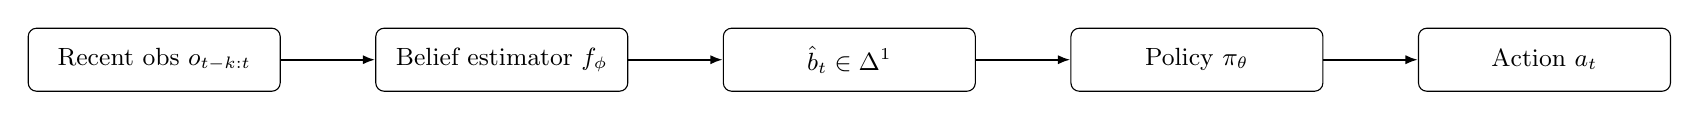
\begin{tikzpicture}[
  box/.style={draw, rounded corners=3pt, align=center, font=\small,
              minimum width=3.2cm, minimum height=0.8cm, inner sep=6pt},
  arr/.style={-{Latex[length=4.5pt]}, thick},
]
  \node[box] (hist) {Recent obs $o_{t-k:t}$};
  \node[box, right=1.2cm of hist] (est)  {Belief estimator $f_\phi$};
  \node[box, right=1.2cm of est]  (bhat) {$\hat{b}_t \in \Delta^1$};
  \node[box, right=1.2cm of bhat] (pol)  {Policy $\pi_\theta$};
  \node[box, right=1.2cm of pol]  (act)  {Action $a_t$};

  \draw[arr] (hist) -- (est);
  \draw[arr] (est)  -- (bhat);
  \draw[arr] (bhat) -- (pol);
  \draw[arr] (pol)  -- (act);
\end{tikzpicture}
\caption{Inference-time architecture once the belief estimator replaces the
         oracle.  $\Delta^1$ denotes the 2-simplex (probability vector over
         two regimes). The estimator $f_\phi$ can be a small LSTM or sliding
         window MLP trained to predict the regime label from public history.}
\label{fig:inferred}
\end{figure}

\paragraph{Training the estimator.}
Generate labeled episodes: for each episode under regime $R \in
\{\textsc{Val}, \textsc{Mom}\}$, the target is the corresponding
one-hot $b^*$.
Train $f_\phi$ to minimize cross-entropy between $\hat{b}_t$ and $b^*$
using only observations $o_{t-k:t}$ (no privileged information).
A \textit{k}-step window of $k=5$ to $k=20$ steps is a reasonable starting
point; the best window length should be selected by held-out classification
accuracy.

\paragraph{Evaluation.}
Compare the inferred-belief PPO agent against:
(a) the v4 belief-blind baseline and
(b) the oracle agent.
The gap between (b) and the inferred-belief agent quantifies how much
accuracy the estimator sacrifices; the gap between (a) and the
inferred-belief agent quantifies the practical gain from the belief module.

% ---------------------------------------------------------------------------
\section{Summary of Proposed Experiments}
% ---------------------------------------------------------------------------

\begin{table}[H]
\centering
\begin{tabular}{lllcc}
\toprule
\textbf{Exp.} & \textbf{Agent type} & \textbf{Obs} & \textbf{New training?} & \textbf{Prerequisite} \\
\midrule
E0 & Oracle heuristic (MR/Mom rule) & $b^*$ visible & No & v1, v4 data \\
E1 & PPO + belief in obs & $[o_t \| b^*]$ & Yes & E0 passes \\
E2 & PPO + belief in reward & $o_t$ only & Yes & E0 passes \\
E3 & PPO + inferred belief $\hat{b}_t$ & $[o_t \| \hat{b}_t]$ & Yes (+ estimator) & E1 or E2 passes gate \\
\bottomrule
\end{tabular}
\caption{Proposed experiment sequence. E0 is a fast sanity check; E1/E2 are the
         oracle variants; E3 is the full belief-aware RL agent.}
\label{tab:experiments}
\end{table}

\bigskip
\noindent
The regime configurations (Table~\ref{tab:regimes}) are fully supported by
existing v1 and v4 sweep data.
No additional simulation runs are required unless E0 fails to show
separation between the two regimes at the heuristic level, in which case
an intermediate-ratio regime (e.g.\ $n_\text{mom}=6$, $r\approx 0.06$)
should be tested to find a cleaner boundary.

\end{document}
